%% LyX 2.2.4 created this file.  For more info, see http://www.lyx.org/.
%% Do not edit unless you really know what you are doing.
\documentclass[english]{article}
\usepackage{lmodern}
\usepackage[T1]{fontenc}
\usepackage[latin9]{inputenc}
\usepackage{geometry}
\geometry{verbose,tmargin=3cm,bmargin=3cm,lmargin=2.5cm,rmargin=2.5cm}
\usepackage{textcomp}
\usepackage{amstext, amsmath}
\usepackage{graphicx}
\graphicspath{{figures/}}

\makeatletter

%%%%%%%%%%%%%%%%%%%%%%%%%%%%%% LyX specific LaTeX commands.
%% Because html converters don't know tabularnewline
\providecommand{\tabularnewline}{\\}

\makeatother

\usepackage{babel}
\begin{document}

\title{3F8: Inference\\
 Short Lab Report}

\author{Shanzi (Monica) Ran}
\maketitle
\begin{abstract}
This lab report records investigations on performance of the logistic classifier and non-linear feature expansion mechanism (RBF). This is implemented using a simple binary categorised dataset, and the performance of classification models is assessed by the comparison of average log-likelihood between training and test data and error probabilities recorded by the confusion matrix. It has been shown in the exercise that while a simple linear classifier fails to capture complexity of the dataset, RBF-transformed input successfully resolves this issue by providing more flexible decision boundaries.
\end{abstract}

\section{Introduction}
In the lab exercise recorded by this report, the properties of a simple logistic classifier is explored by applying it to a binary dataset, followed by investigation of metrics like average log-likelihood and confusion matrices.
As classification is a fundamental task of machine learning, this investigation is necessary for the understanding of capabilities of different models and parameters.
In this report, this classifier architecture is investigated both theoretically and practically, while non-linear feature expansion techniques are also explored as an alternative method to improve the classification performances.
\section{Exercise a)\label{sec:Exercise-a}}

In this exercise we have to consider the logistic classication model
(aka logistic regression) and derive the gradients of the log-likelihood
given a vector of binary labels $\mathbf{y}$ and a matrix of input
features $\mathbf{X}$. The gradient of the log-likelihood can be
writen as
\begin{align*}
    \frac{\partial\mathcal{L}(\beta)}{\partial\beta} &= \frac{\partial}{\partial\beta} \prod_{n=1}^{N} log\{\sigma(\beta^T \tilde{x}^{(n)})^{y^{(n)}} (1-\sigma(\beta^T \tilde{x}^{(n)}))^{1-y^{(n)}}\} \\
    &= \sum_{n=1}^{N} \{y^{(n)}\frac{\partial}{\partial\beta}log\{\sigma(\beta^T \tilde{x}^{(n)})\} + (1-y^{(n)})\frac{\partial}{\partial\beta}log\{1-\sigma(\beta^T \tilde{x}^{(n)})\}\}
\end{align*}

Using derivative results (substituting $ z = \beta^T \tilde{x}^{(n)} $):
\begin{align*}
    \frac{\partial}{\partial z} \log \sigma(z) &= \frac{1}{\sigma(z)}\sigma(z) (1 - \sigma(z)) = 1 - \sigma(z) \\
    \frac{\partial}{\partial z} \log (1 - \sigma(z)) &= \frac{1}{1 - \sigma(z)} (-\sigma(z) (1 - \sigma(z))) = -\sigma(z) \\
\end{align*}

We can then write:
\begin{align*}
    \frac{\partial\mathcal{L}(\beta)}{\partial\beta} &= \sum_{n=1}^{N} \{ y^{(n)} (1 - \sigma(\beta^T \tilde{x}^{(n)})) \tilde{x}^{(n)} - (1 - y^{(n)}) \sigma(\beta^T \tilde{x}^{(n)}) \tilde{x}^{(n)} \} \\  
    &= \sum_{n=1}^{N} \{y^{(n)} - \sigma(\beta^T \tilde{x}^{(n)}) \} \tilde{x}^{(n)}
\end{align*}

\section{Exercise b)}

In this exercise we are asked to write pseudocode to estimate the
parameters $\beta$ using gradient ascent of the log-likelihood. Our
code should be vectorised. The pseudocode to estimate the parameters
$\beta$ is shown below:
\begin{verbatim}
Function estimate_parameters:

   Input:  feature matrix X, labels y
   Output: vector of coefficients b
	
    max_iter = 1000 # maximum number of iterations set to avoid infinite training
    eta = 0.01 # learning rate (choice explained below)
    b = zeros(D) # initialise coefficients vector with dimention D
    for iter in range(max_iter):
        grad_old = X.T @ (y - sigmoid(X @ b)) # calculate old gradient
        b_new = b + eta * grad_old # gradient ascent
        if norm(b_new - b) == 0: # check whether has reached local maximum
            break
        b = b_new
   return b
\end{verbatim}
The learning rate parameter $\eta$ is chosen to avoid both divergence due to too large $\eta$ and slow convergence due to too small $\eta$.
Therefore, it is here set to the widely accepeted default value of $0.01$.
\section{Exercise c)}

In this exercise we visualise the dataset in the two-dimensional input
space displaying each datapoint's class label. The dataset is visualised
in Figure \ref{fig:data_visualisation}. By analising Figure \ref{fig:data_visualisation}
we conclude that a linear classifier would not be able to perform the classification task satisfactorily due to the complex structure of the dataset. 

\begin{figure}
\begin{centering}
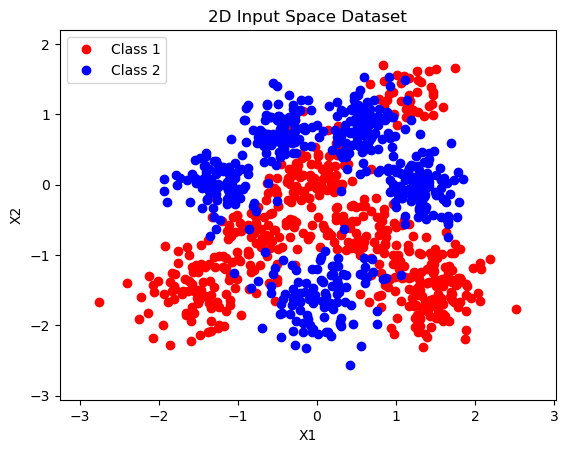
\includegraphics[width=0.3\paperwidth]{c.png}
\par\end{centering}
\caption{Visualisation of the data.\label{fig:data_visualisation} }
\end{figure}


\section{Exercise d)}

In this exercise we split the data randomly into training and test
sets with 800 and 200 data points, respectively. The pseudocode from
exercise a) is transformed into python code as follows:
\begin{verbatim}
    sigmoid_value = predict(X_tilde_train, w)

    gradient = X_tilde_train.T @ (y_train - sigmoid_value)

    w = w + alpha * gradient
\end{verbatim}

We then train the classifier using this code. We fixed the learning
rate parameter to be $\eta=0.001$ to inhibit oscillations. The average log-likelihood on the
training and test sets as the optimisation proceeds are shown in Figure
\ref{fig:learning_curves}. By looking at these plots we conclude
that for the given ratio of dataset split, the average log-likelihood value on the training dataset converges to a higher value than that of the test dataset. This difference is not large though, which is suspected to be the consequence of too much training data.

Figure \ref{fig:learning_curves} displays the visualisation of the
contours of the class predictive probabilities on top of the data.
This figure shows that the linear classifier model does not separate the categories clearly when applied to the original dataset. Therefore, alternative non-linear feature expansion methods like the RBF is explored in later sections of this report.

\begin{figure}
\begin{centering}
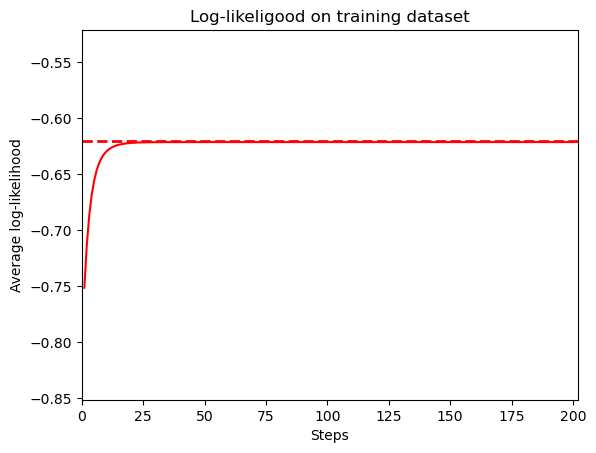
\includegraphics[width=0.3\paperwidth]{d1.png}\hspace{1cm}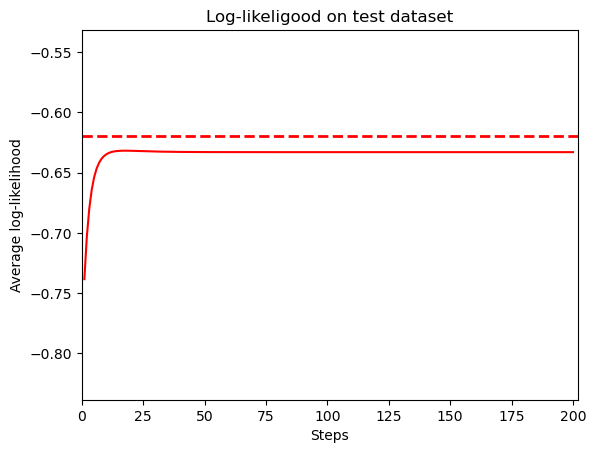
\includegraphics[width=0.3\paperwidth]{d2.png}
\par\end{centering}
\caption{Learning curves showing the average log-likelihood on the training
(left) and test (right) datasets.\label{fig:learning_curves} }
\end{figure}

\begin{figure}
\begin{centering}
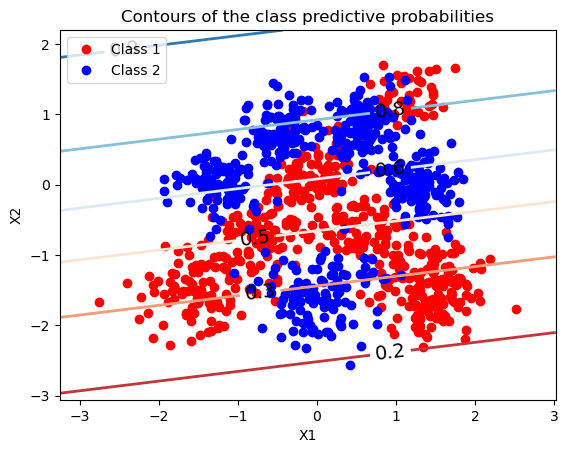
\includegraphics[width=0.3\paperwidth]{d3.png}
\par\end{centering}
\caption{Visualisation of the contours of the class predictive probabilities.\label{fig:data_visualisation-1} }
\end{figure}


\section{Exercise e)}

The final average training and test log-likelihoods are shown in Table
\ref{tab:average_ll}. These results indicate that the classifier performs better with the training dataset than with the test dataset, which is reasonble result. The 2x2 confusion
matrices on the and test set is shown in Table \ref{tab:confusion_test}.
By analising this table, we conclude that  the probability of error for linear classification is approximately equal for the two classes, with an value $P_e \approx 0.28$ (taking average). This error probability agrees with expectation that pure linear classification is not sufficiently complex and accurate for the dataset used.

\begin{table}
\centering{}%
\begin{minipage}[t]{0.49\columnwidth}%
\begin{center}
\begin{tabular}{c|c}
\textbf{Avg. Train ll} & \textbf{Avg. Test ll}\tabularnewline
\hline 
$-0.627$ & $-0.609$\tabularnewline
\hline 
\end{tabular} 
\par\end{center}
\caption{Average training and test log-likelihoods.\label{tab:average_ll}}
%
\end{minipage}%
\begin{minipage}[t]{0.49\columnwidth}%
\begin{center}
\begin{tabular}{cc|c|c}
 & \multicolumn{1}{c}{} & \multicolumn{1}{c}{$\hat{y}$} & \tabularnewline
 &  & 0 & 1\tabularnewline
\cline{2-4} 
$y$ & 0 & $0.7075$ & $0.2925$\tabularnewline
\cline{2-4} 
 & 1 & $0.2753$ & $0.7247$\tabularnewline
\cline{2-4} 
\end{tabular} 
\par\end{center}
\caption{Confusion matrix on the test set.\label{tab:confusion_test}}
%
\end{minipage}
\end{table}


\section{Exercise f)}

We now expand the inputs through a set of Gaussian radial basis functions
centred on the training datapoints. We consider widths $l=\{0.01,0.1,1\}$
for the basis functions. We fix the learning rate parameter to be
$\eta=\{0.01,0.01,0.0001\}$ for each $l=\{0.01,0.1,1\}$, respectively.
Figure \ref{fig:contours_l} displays the visualisation of the contours
of the resulting class predictive probabilities on top of the data
for each choice of $l=\{0.01,0.1,1\}$.

\begin{figure}
\begin{centering}
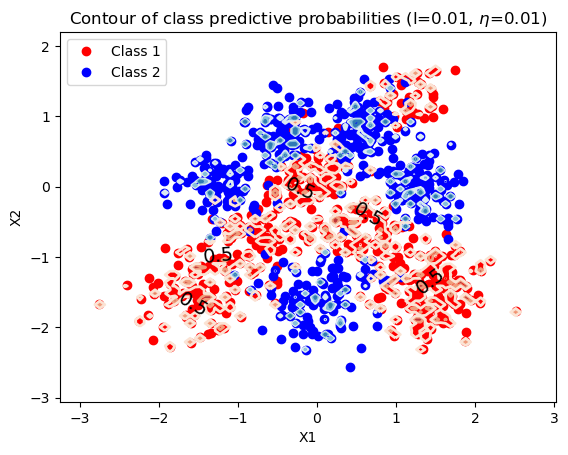
\includegraphics[width=0.32\textwidth]{g1.png}\hspace{0.15cm}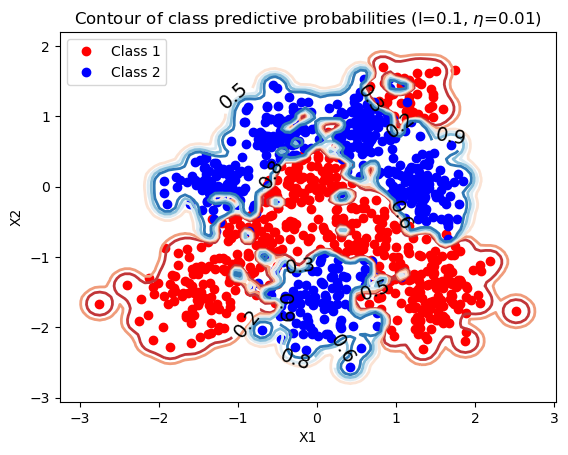
\includegraphics[width=0.32\textwidth]{g2.png}\hspace{0.15cm}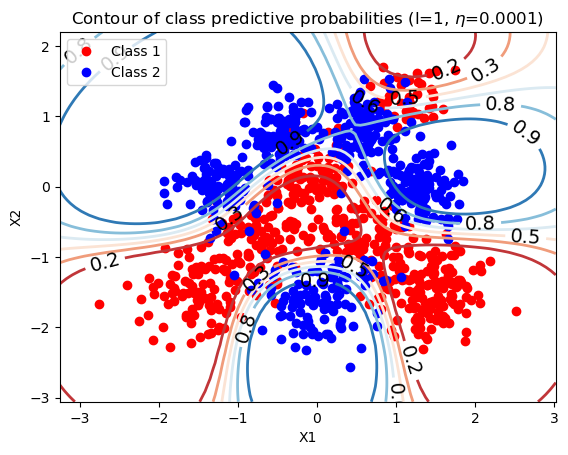
\includegraphics[width=0.32\textwidth]{g3.png}
\par\end{centering}
\caption{Visualisation of the contours of the class predictive probabilities
for $l=0.01$ (left), $l=0.1$ (middle), $l=1$ (right).\label{fig:contours_l} }
\end{figure}


\section{Exercise g)}

The final final training and test log-likelihoods per datapoint obtained
for each setting of $l=\{0.01,0.1,1\}$ are shown in tables \ref{tab:avg_ll_l_001},
\ref{tab:avg_ll_l_01} and \ref{tab:avg_ll_l_1}. These results indicate
that as $l$ value increases, the classifier performance on training dataset gets worse, but it also exhibits better adaptation to unobserved test dataset, which indicate that although the model is less sensitive and accurate when identifying details, it has successfully prevented overfitting as depicted in Fig~\ref{fig:contours_l}. The 2 \texttimes{} 2 confusion matrices for the three models
trained with $l=\{0.01,0.1,1\}$ are show in tables \ref{tab:conf_l_001},
\ref{tab:conf_l_01} and \ref{tab:conf_l_1}. After analysing these
matrices, we can say that although $l=0.01$ and $l=1$ settings produce good classification results for one of the categories, it is $l=0.1$ that gives the most balanced confusion matrix, where the error probability of each category is approximately the same value $0.05$. When we compare these results to those
obtained using the original inputs we conclude that all three models produce better classification results than that of the initial model. Hence, non-linear expansion of features like RBF could significantly boost the performance of linear classifier regardless of RBF settings. Combining with decision boundary contours displayed in Fig~\ref{fig:contours_l}, it is then concluded that non-linear feature expansion is a useful technique when classifying datasets with complex features.

\begin{table}
\centering{}%
\begin{minipage}[t]{0.3\textwidth}%
\begin{center}
\begin{tabular}{c|c}
\textbf{Avg. Train ll} & \textbf{Avg. Test ll}\tabularnewline
\hline 
$-0.013$ & $-0.664$\tabularnewline
\hline 
\end{tabular}\caption{Results for $l=0.01$\label{tab:avg_ll_l_001}}
\par\end{center}%
\end{minipage}\hspace{0.5cm}%
\begin{minipage}[t]{0.3\textwidth}%
\begin{center}
\begin{tabular}{c|c}
\textbf{Avg. Train ll} & \textbf{Avg. Test ll}\tabularnewline
\hline 
$-0.036$ & $-0.463$\tabularnewline
\hline 
\end{tabular}\caption{Results for $l=0.1$\label{tab:avg_ll_l_01}}
\par\end{center}%
\end{minipage}\hspace{0.5cm}%
\begin{minipage}[t]{0.3\textwidth}%
\begin{center}
\begin{tabular}{c|c}
\textbf{Avg. Train ll} & \textbf{Avg. Test ll}\tabularnewline
\hline 
$-0.244$ & $-0.233$\tabularnewline
\hline 
\end{tabular}\caption{Results for $l=1$\label{tab:avg_ll_l_1}}
\par\end{center}%
\end{minipage}
\end{table}

\begin{table}
\centering{}%
\begin{minipage}[t]{0.33\textwidth}%
\begin{center}
\begin{tabular}{cc|c|c}
 & \multicolumn{1}{c}{} & \multicolumn{1}{c}{$\hat{y}$} & \tabularnewline
 &  & 0 & 1\tabularnewline
\cline{2-4} 
$y$ & 0 & $0.996$ & $0.004$\tabularnewline
\cline{2-4} 
 & 1 & $0.174$ & $0.826$\tabularnewline
\cline{2-4} 
\end{tabular} 
\par\end{center}
\caption{Conf. matrix $l=0.01$.\label{tab:conf_l_001}}
%
\end{minipage}%
\begin{minipage}[t]{0.33\textwidth}%
\begin{center}
\begin{tabular}{cc|c|c}
 & \multicolumn{1}{c}{} & \multicolumn{1}{c}{$\hat{y}$} & \tabularnewline
 &  & 0 & 1\tabularnewline
\cline{2-4} 
$y$ & 0 & $0.945$ & $0.055$\tabularnewline
\cline{2-4} 
 & 1 & $0.049$ & $0.951$\tabularnewline
\cline{2-4} 
\end{tabular} 
\par\end{center}
\caption{Conf. matrix $l=0.1$.\label{tab:conf_l_01}}
%
\end{minipage}%
\begin{minipage}[t]{0.33\textwidth}%
\begin{center}
\begin{tabular}{cc|c|c}
 & \multicolumn{1}{c}{} & \multicolumn{1}{c}{$\hat{y}$} & \tabularnewline
 &  & 0 & 1\tabularnewline
\cline{2-4} 
$y$ & 0 & $0.887$ & $0.113$\tabularnewline
\cline{2-4} 
 & 1 & $0.079$ & $0.921$\tabularnewline
\cline{2-4} 
\end{tabular} 
\par\end{center}
\caption{Conf. matrix $l=1$.\label{tab:conf_l_1}}
%
\end{minipage}
\end{table}


\section{Conclusions}
In this lab exercise, the logistic regression model is explored as a method for binary data classification. It has been observed that although simple implementation of the linear model fails to accurately capture the complexity of the dataset used, pre-processing the dataset by RBF feature expansion is generally helpful in improving the probability of error.
It should also be noted how a larger RBF length scale $l$ will positively affect the model by preventing overfitting at the cost of classification precision. However, this conclusion is yet to be complete as more non-linear filtering methods should be investigated and compared to the optimal performance. The dataset used in this exercise is also relatively small, so verbatim implementation for larger datasets could also be a concern subject to future explorations.

\end{document}
